% !TEX root = ./main.tex
\chapter{Introduction}

This chapter discusses fundamental properties of aerosols and computational modeling techniques which motivate this thesis. A description of atmospheric aerosols and the challenges associated with capturing the complexity of aerosol properties and their environmental feedbacks is discussed. Additionally, numerical modeling treatments for aerosols are presented along with approaches to improve the characterization of aerosol complexity. Finally, research questions are presented which outline primary avenues of inquiry for this thesis.  

\section{The complexity of aerosols and environmental feedbacks}

An aerosol is a collection of particles composed of one or more chemical species that are suspended in a fluid or gas. In the atmosphere, aerosol particles vary considerably in terms of their physical properties such as size, composition, and origin. Additionally, the chemical, thermodynamic, and radiative properties of aerosol particles can alter the state of the aerosol and the surrounding environment through numerous feedback mechanisms. In turn, aerosol particles exhibit a complex, non-linear coupling with the environment that spans broad spatial and temporal scales.

Aerosol particles are typically measured by their diameter where spherical morphology is assumed. The smallest particles have diameters on the order of 1 nm and are produced via the nucleation of low-volatility vapors. On the opposite extreme of particle sizes, the largest particle diameters can exceed 100 $\upmu$m. In total, aerosols span approximately five orders of magnitude. To capture the broad scale of particle diameters that may be present in a population of aerosol particles, aerosol size distributions often represent the number concentration of particles as a function of the logarithm of particle diameter. The particle size distribution may be represented by multiple modes---lognormal size distributions---that are differentiated by the characteristics of particles within each mode, including growth and removal mechanisms. Typically, three distinct modes are present in a particle size distribution: the nucleation, accumulation, and coarse mode. 

Nucleation mode particles are up to 20 nm in diameter and undergo rapid growth as gas-phase species condense onto the particle surface or as particles inelastically collide through coagulation. They are removed from the nucleation mode by growth within \hl{XX} time into the accumulation mode, which spans particle diameters from 0.1 $\upmu$m to 2 $\upmu$m . In addition to particles that enter the accumulation mode through growth by condensation or coagulation, particles may be released directly into the accumulation mode via primary emissions. Removal mechanisms such as wet and dry deposition are least efficient in the accumulation mode, allowing particles to remain suspended in the atmosphere for days to weeks. Particles in the coarse mode have diameters exceeding 2 $\upmu$m  and are produced by mechanical processes such as abrasion and the resuspension of dust. Due to their size, particles in the coarse mode are rapidly removed by gravitational settling within minutes to hours. This multi-modal description of the aerosol size distribution points to the inherent complexity of aerosol population dynamics---production, growth, and removal mechanisms differ considerably by particle size. 

As noted, production mechanisms vary across aerosol modes (e.g., nucleation of low-volatility vapors, emission of primary aerosol  into the accumulation mode, resuspension of coarse particles, etc.). These processes typically involve different chemical species. For example, whereas volatile organic compounds (VOCs) such as isoprene and other organic carbon (OC) species may undergo oxidation reactions which lower their volatility and promote particle nucleation, particles released directly into the accumulation or coarse mode as primary aerosol may consist of either organics that are produced during combustion such as black carbon (BC) or inorganics such as sea salt spray, mineral dust, \hl{[other species]}. \hl{Here its worth acknowledging contribution of precursor emissions to chemical aging, secondary production of aerosol-phase matter, changes to aerosol mixing state, etc.}. As a result, aerosol particles are compositionally diverse. 

In addition to diversity in the composition of aerosol particles across the size distribution, aerosol populations also exhibit spatiotemporal variations which alter the local structure and composition of the aerosol. The geographic distribution of emission sources, varied land use, and topography lead to spatial heterogeneities in the emission of gas-phase precursors and primary aerosols. Additionally, temporal trends alter the meteorological state of the atmosphere and the concentration of reactive gas or aerosol-phase species. For instance, diurnal variation in the structure of the boundary layer due to surface heating determines the strength of vertical transport and mixing of primary aerosol or reactive gas-phase species. \hl{[Could talk about photolysis]}. Furthermore, the timing of emissions may play a crucial role in determining whether a chemical reaction will take place; reactive species must be present in the same space and time to undergo reaction.

\cite{seinfeld_atmospheric_1998}

\section{Spatial heterogeneity of aerosols}

\begin{itemize}

\item Spatial heterogeneity of surface heterogeneities impacts the evolution of the atmospheric state
\begin{itemize}
\item Joint modeling and observation based studies like Fast et al. 2019 “HI-SCALE” heterogeneities in soil moisture were critical to cloud structure and the development of deeper convecting clouds. Modeling studies showed that under scenarios with smoothly varying soil moisture, clouds did not develop into open cell, deep convective cumulus capable of precipitating and instead were characterized by shallow, uniform non-precipitating clouds. 
\item Lee et al. 2018 conducted an idealized LES study in which surface heat fluxes (including both sensible and latent heat flux) were prescribed by checkerboard patterns of ranging spatial heterogeneity (most heterogeneous being the lowest frequency checkerboard pattern--largest pattern length scale--and least heterogeneous being the highest frequency patterns--smallest pattern length scale). They found that secondary circulation developed under scenarios with the highest spatial heterogeneity and minimal background winds (less than 2 \si{m.s^{-1}}). This circulation was responsible for transporting moisture from checkerboard regions with greater latent heat flux to drier regions with lesser latent heat flux. 
\end{itemize}

\item Aerosols have shown to also be highly variable:
\begin{itemize}
\item Examples: Urban, rural, maritime, etc. (variability in composition, concentration). See Seinfeld and Pandis for some discussion of typical conditions in each region.
\end{itemize}

\item Existing studies looking at spatial heterogeneity of aerosols
\begin{itemize}
\item Fast et al. 2022 (properties)
\item Hassan et al. 2023 (emissions)
\item Franklin et al. 2018
\end{itemize}

\item Impacts on aerosol processes: non-linear, concentration dependent processes
\begin{itemize}
\item Coagulation
\item Chemistry
\begin{itemize}
\item Present body of literature investigates predominantly gas-phase chemistry (e.g., isoprene-OH reaction) and contribution of chemical segregation due to turbulence and spatial distribution of reactive species
\end{itemize}
\item These processes alter the radiative and hygroscopic properties of the aerosol 
\end{itemize}

\item Representation of aerosol spatial heterogeneity in models
\begin{itemize}
\item Lack of resolution, impact of sub-grid scale variability on aerosol properties (Radiative properties, CCN concentrations)
\begin{itemize}
\item Lin et al. 2017 find that aerosol (mass I think) SGV over the pacific ocean within a typical GCM grid cell is 15\% near the surface and as high as 50\% in the free troposphere. (this could also be cited in the paragraph above on variability of aerosols).
\item Weigum et al. 2016 look at the effect of SGV on AOD and CCN by comparing WRF-Chem runs at 80 km resolution against 10 km resolution and find an underestimation of AOD by 13\% and an overestimation of CCN by 27\%. They find gas-phase chemistry and aerosol water uptake are processes which are most affected.
\item Qian et al. 2010 (study over mexico, contribution of emissions to SGV)
\item Gustafason et al. 2011 (similar to Qian 2010, radiative effects)
\item Crippa et al. 2017
\end{itemize}
\item Attempts at parameterizations (adaptive grids, plume in grid modeling, coagulation parameterizations, PDF-based methods, stochastic fields, etc.)
\end{itemize}

\end{itemize}

\section{Impacts of aerosols on climate}

\begin{itemize}

\item Aerosol-radiative effects
\begin{itemize}
\item Absorption and scattering of radiation alters the stability of the atmosphere due to warming/cooling
\item Aerosols alter large scale circulation. For example, higher aerosol concentrations due to anthropogenic activity in the northern hemisphere results in global-scale heterogeneity. Fan et al. 2016 (via Ming and Ramaswamy 2011) note that this weakens the northern branch of the Hadley circulation, resulting in an energy flux from the southern hemisphere towards the north.  
\end{itemize}

\item Aerosol-cloud interactions
\begin{itemize}
\item Indirect effects - Twomey, etc.
\item Impacts on cloud type and evolution
\begin{itemize}
\item Warm rain mechanism well understood
\item Thermodynamic invigoration due to increased CCN for deep-convective clouds (mechanism much more complicated, still contested)
\item Have been shown to promote formation of open cells
\end{itemize}
\item Radiative forcing due to ACI and sources of uncertainty
\begin{itemize}
\item One source of uncertainty is aerosol representation in models
\end{itemize}
\end{itemize}

\end{itemize}

\section{Treatment of aerosols across modeling frameworks}

\begin{itemize}

\item Simplified bulk, modal, sectional treatments
\begin{itemize}
\item Use in regional, global scale models
\item Consequences of simplified treatment on representation of CCN concentrations, etc. 
\end{itemize}
\item Particle resolved aerosol modeling
\item Transport representation 
\begin{itemize}
\item Large scale models use RANS and thus cannot resolve turbulence and associated heterogeneities in gas, aerosol concentrations
\item LES - adoption for modeling aerosols is still nascent, some examples like UCLALES-SALSA, DALES have been used to evaluate aerosol-cloud interactions, but none leverage a high-resolution particle resolved aerosol treatment
\end{itemize}

\end{itemize}

\section{Objectives of this thesis}

\begin{itemize}

\item Primary science questions
\begin{itemize}
\item Impacts of emissions spatial heterogeneity on aerosol processes (e.g., coagulation, chemistry, etc.)?
\item Impacts of emissions spatial heterogeneity on aerosol properties (e.g., composition, concentration, hygroscopicity)? 
\item How is the impact of spatial heterogeneity on aerosols modulated by changes to the composition of emissions?
\item How does emissions spatial heterogeneity alter the activity of CCN?
\end{itemize}

\item Development of a framework for evaluating spatial heterogeneity impact on aerosol properties, including CCN activity
\begin{itemize}
\item Transport vs. aerosol treatment graph 
\item Future extension could quantify the structural uncertainty for the representation of aerosols (properties, ccn activity, etc.) in coarser resolved models such as regional and global scale models that use modal/sectional aerosol treatments and parameterize turbulence 
\end{itemize}

\end{itemize}

\begin{figure}[h]
	\centering
	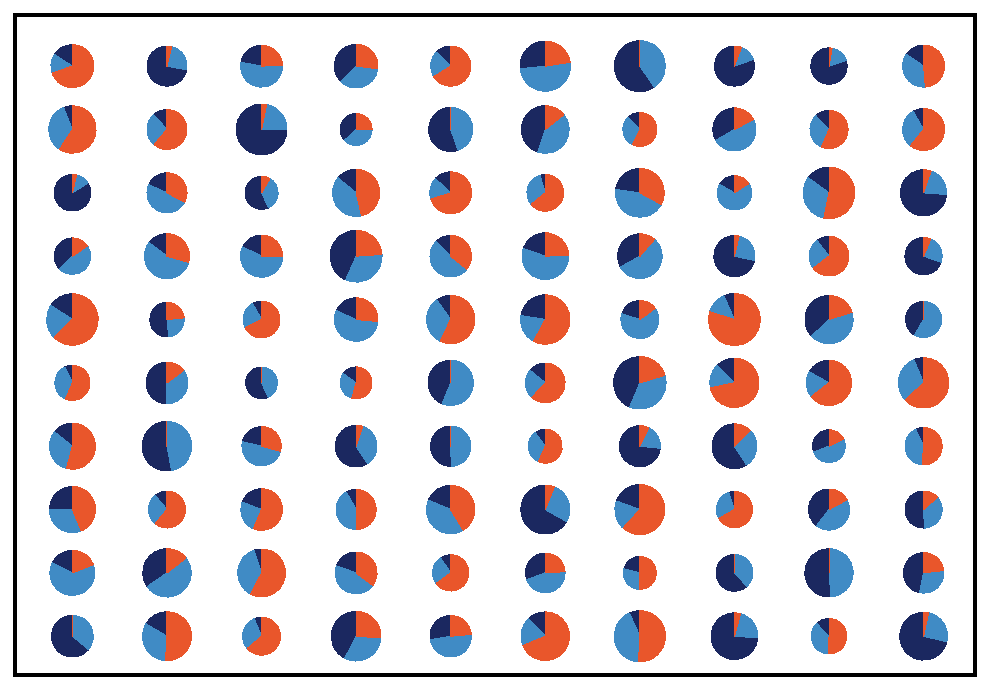
\includegraphics[width=\textwidth]{particle-resolved-model.pdf}
	\caption{Cartoon representation of a particle resolved model}
	\label{fig:test}
\end{figure}

\begin{table}[h!]
\centering
\begin{tabular}{||c c c c||} 
 \hline
 Col1 & Col2 & Col2 & Col3 \\ [0.5ex] 
 \hline\hline
 1 & 6 & 87837 & 787 \\ 
 2 & 7 & 78 & 5415 \\
 3 & 545 & 778 & 7507 \\
 4 & 545 & 18744 & 7560 \\
 5 & 88 & 788 & 6344 \\ [1ex] 
 \hline
\end{tabular}
\caption{Table to test captions and labels.}
\label{table:1}
\end{table}